\section{Project Background}
\subsection{Measuring the Health of Bridges}


\subsection{Wireless Sensor Networks}
Wireless Sensor Networks (WSNs) are simple, low-cost networks that primarily consist of nodes and a base station \cite{WSN-WaterQual}. WSN nodes usually comprise of some sensing or measuring capability acting as the physical layer, and relay this information via uplink to a base station for processing and then to a network server acting as the network layer. From here, the API from a network cloud service can be used to create GUI's and other applications for researchers and consumers which acts as the application layer. 

Innovating many field of industry and research, these distributed networks of nodes have been valuable in many contexts. For example, the use of ZigBee communication technology for air pollution monitoring \cite{ZigBeeAirPolution} and the use of Bluetooth for communication between end-devices measuring temperature, luminance, carbon dioxide and humidity for energy-saving establishments \cite{BTenergySaving}. Although these WSNs have worked in the past, the future of this technology lies in developing systems that have high scalability and range, something that ZigBee and Bluetooth inherently lack. Cellular and satellite technology are alternate approaches that offer extremely high data rates and range, however these technologies are not practical to implement in most situations due to exceedingly high costs. 

\subsection{LoRa and LoRaWAN}
Low Power Wide Area Network (LPWAN) is a communication technology that boasts similar ranges to satellite (WHAT RANGE) but with lower data rate than ZigBee. The trade-off is extremely low energy consumption and deployment / maintenance cost \cite{IOTandLORAWAN-SmartFarm}. Figure \ref{IOTandLORAWAN-SmartFarm-Figure1} displays the fundamental differences between each of the mentioned communication technologies. It is clear that LP-WAN immediately has many more use cases for applications that require long range but are not as concerned with data resolution or packet density. The physical layer end devices are designed to be discrete and the low maintenance cost and energy consumption allow them to be placed and forgotten for up to ten years CITE THE 10 YEARS ----------------.

\begin{figure}[h]
	\centering 
	\caption{Comparison of main IoT enabling communication technologies in terms of range, data rate, energy consumption, and costs. \cite{IOTandLORAWAN-SmartFarm}}
	\label{IOTandLORAWAN-SmartFarm-Figure1}
	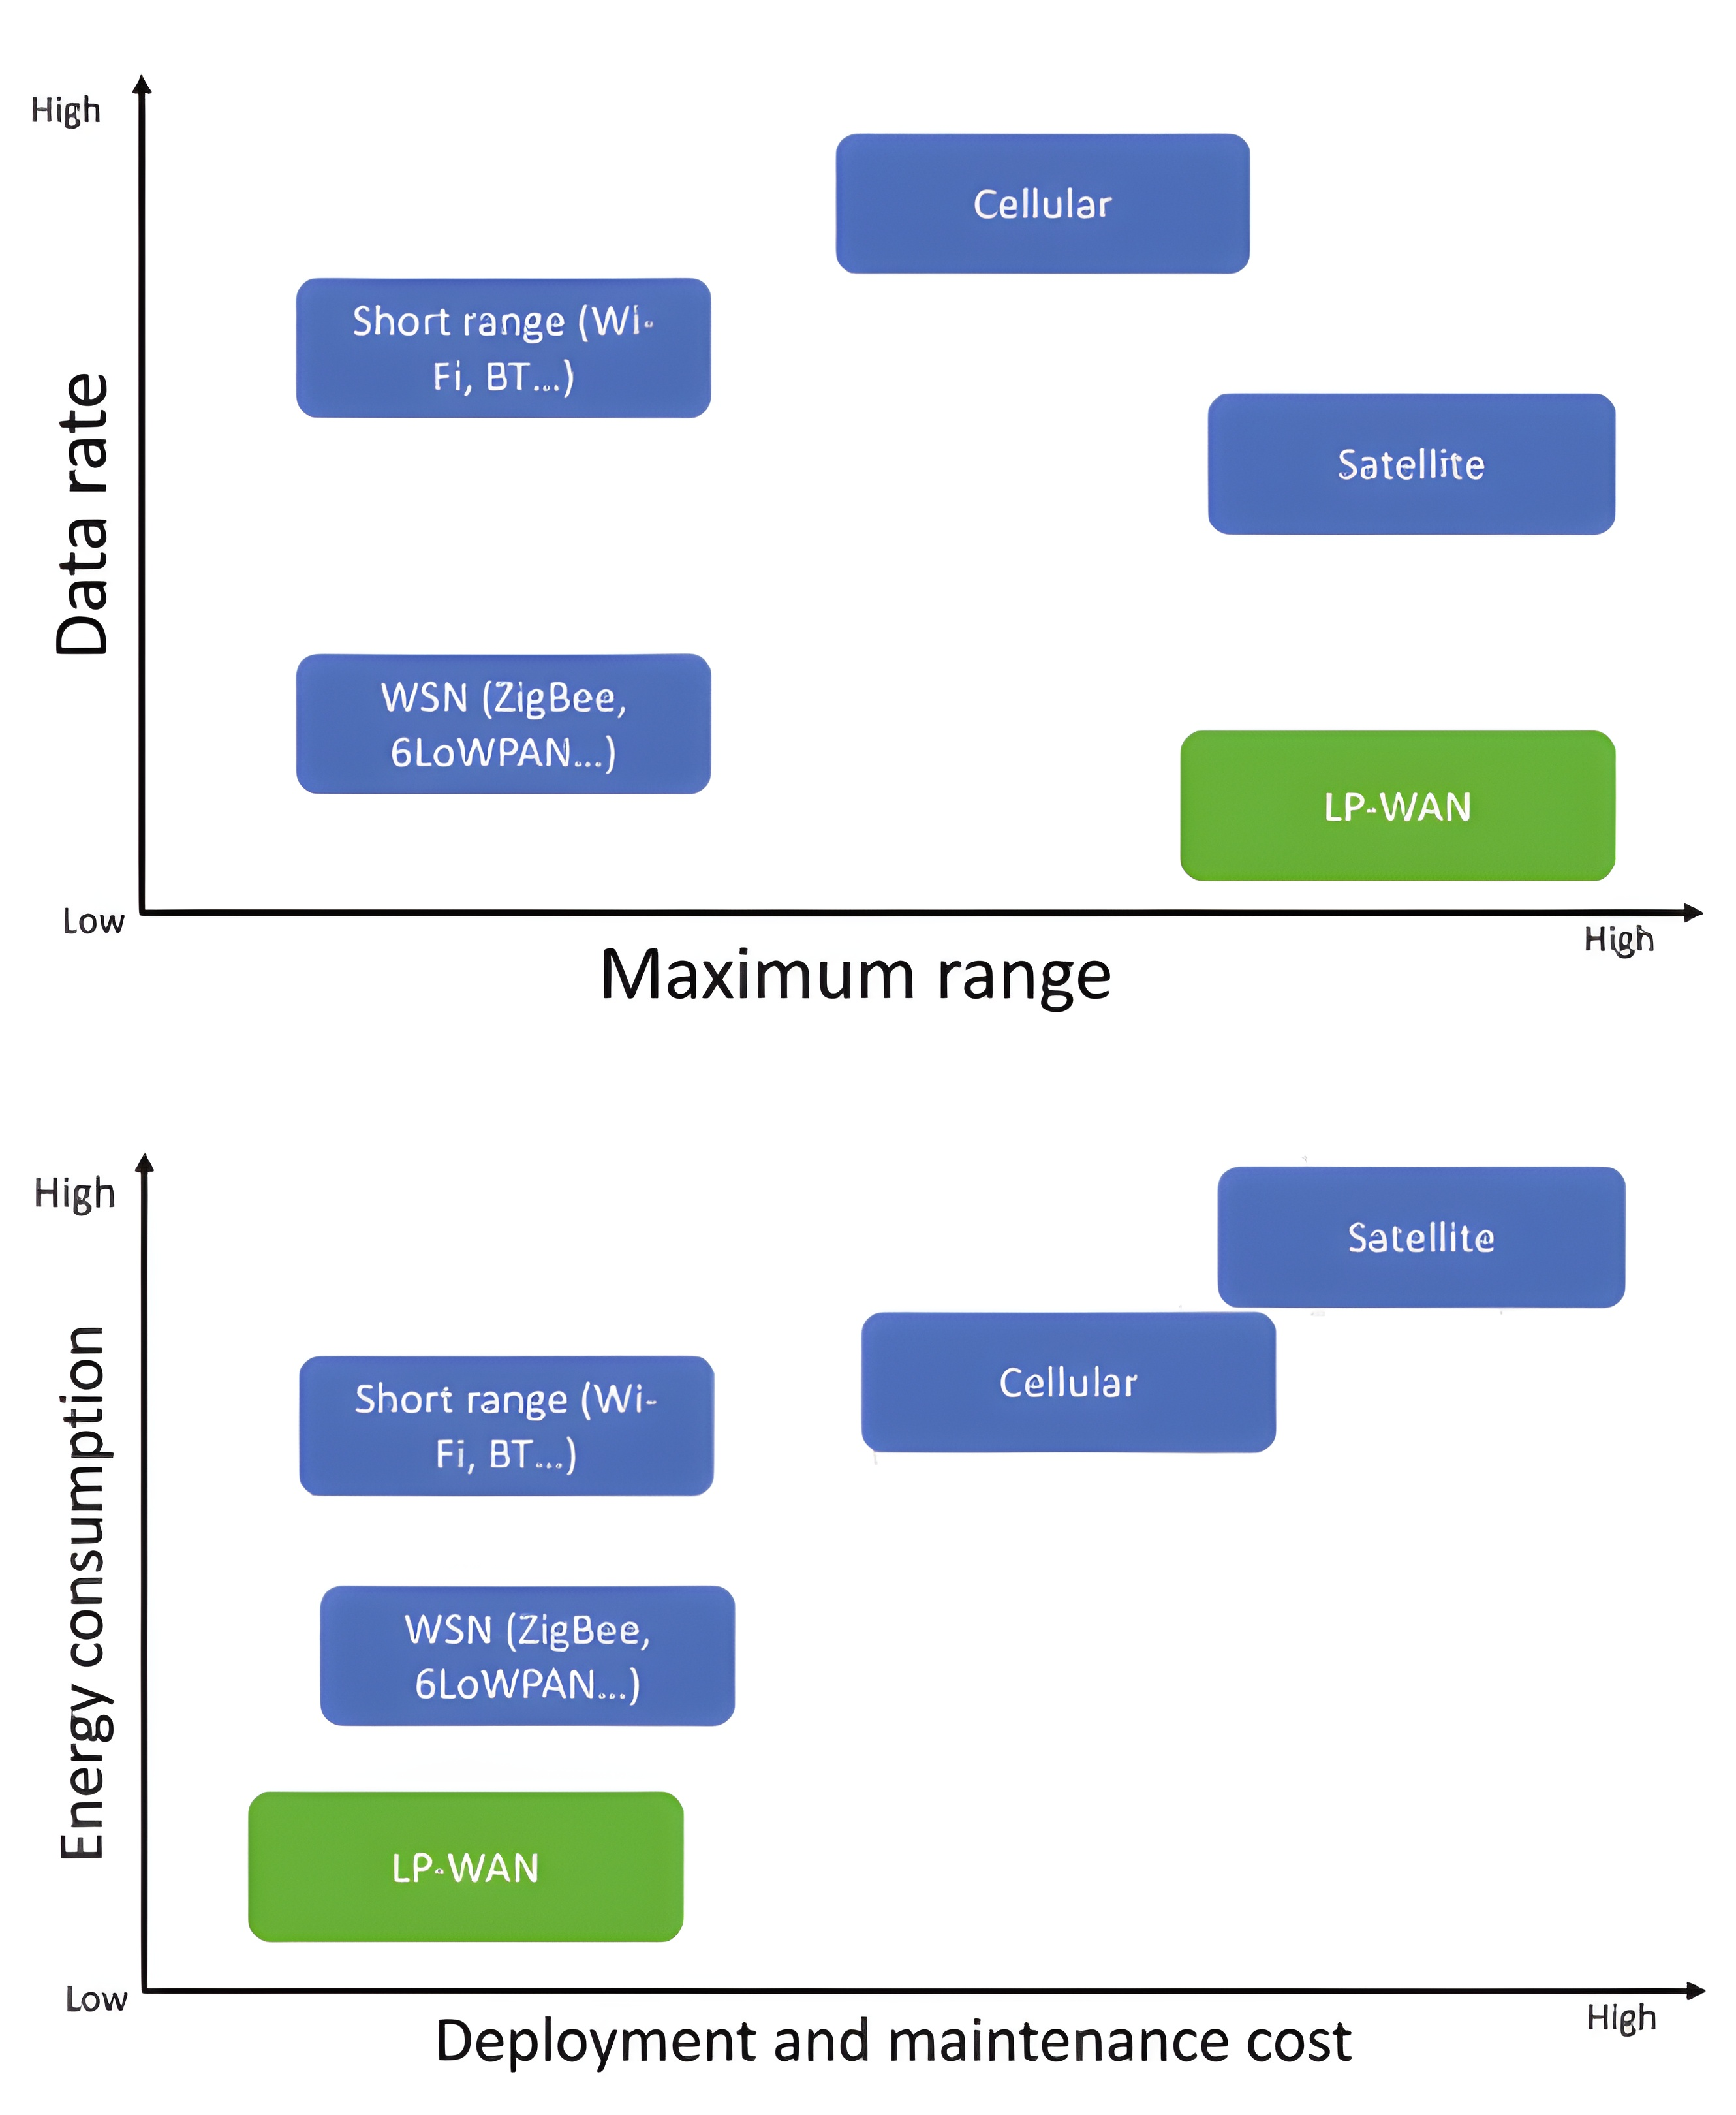
\includegraphics[scale=0.1]{Sections/Introduction/LP-WAN-Range.jpg}
\end{figure}

Long Range (LoRa) and Long Range Wide Area Network (LoRaWAN) technology is a form of LP-WAN communication technology developed by DEVELOPED BY WHO ----------- AND CITE. The configuration of WSNs have typically been based on the deployment of Wireless Personal Area Network (WPAN) or Low Power Wide Area Network (LPWAN) standards, 
where nodes are setup in a mesh layout using one of the afore-mentioned short-range communication protocols such as ZigBee and Bluetooth \cite{WSN-WaterQual}. The main implication with these protocols is that the mesh implementation inherently bottlenecks scalability due to exponentially increasing network requirements and power consumption \cite{IOTandLORAWAN-SmartFarm}. LoRaWAN is a solution to implementing an LPWAN system with minimal complexity and scalability due to its star of stars configuration ------- WHAT IS STAR OF STARS AND WHY IS IT BETTER AND CITE. LoRa by definition is a chirp spread spectrum (CSS) modulation technique developed by Cycleo offering a Medium Access Control (MAC) layer protocol and operates on the `licence-free region-dependent industrial, scientific, and medical (ISM) frequncy bands' \cite{IOTandLORAWAN-SmartFarm}. In Australia the operational ISM band for LoRa is between 915 and 928 MHz. LoRaWAN is the ideal technology for agritulcutral and regional purposes due to its long range, low power long lifetime and scalability. 

\section{Internet of Things}
The Internet of Things (IoT) is an `interconnected network of things' \cite{IoT}, where `things' in this context is defined as an end-device with WSN type capability. The IoT architecture comprises of six-layers, the coding layer, perception layer, network layer, middle-ware layer, application layer and business layer \cite{IoT}. Thus to create this IoT architecture for research purposes the first five layers need to be implemented. LoRa end-devices act as the physical layer encompassing the coding and perception layer. The coding layer involves associating unique ID specifiers to each end device \cite{IoT} and the perception layer is involved with on-board sensing and data acquisition. The network layer is a relay of this perceptual information to a gateway, and the middle-ware layer is the IoT cloud platform that facilitates these connections and receives information from the network layer. The application layer involves pulling the API or information from the network layer and developing apps or graphical user interfaces (GUIs) to display the data. The Things Network (TNN) is an open-source LoRaWAN network server used to construct IoT cloud applications with end-to-end encryption and secure communication \cite{LoRaWAN-Smart-Infrastructure-Monitoring}. TNN exists on the middle-ware layer and can be used to deploy an IoT architecture using LoRa end-devices in the coding and perception layer, and utilize the LoRaWAN communication protocol in the network layer. TNN offers a console and API to develop applications that serve as the architecture's application layer. Figure \ref{LoRa-IOT-Example} displays an example of an IoT architecture using WSN nodes, a LoRaWAN gateway, cloud storage and user devices. 

\begin{figure}[h]
	\centering
	\caption{The LoRa network architecture for agriculture area. \cite{LoRaWAN-WSN-Agricultual-Application}}
	\label{LoRa-IOT-Example}
	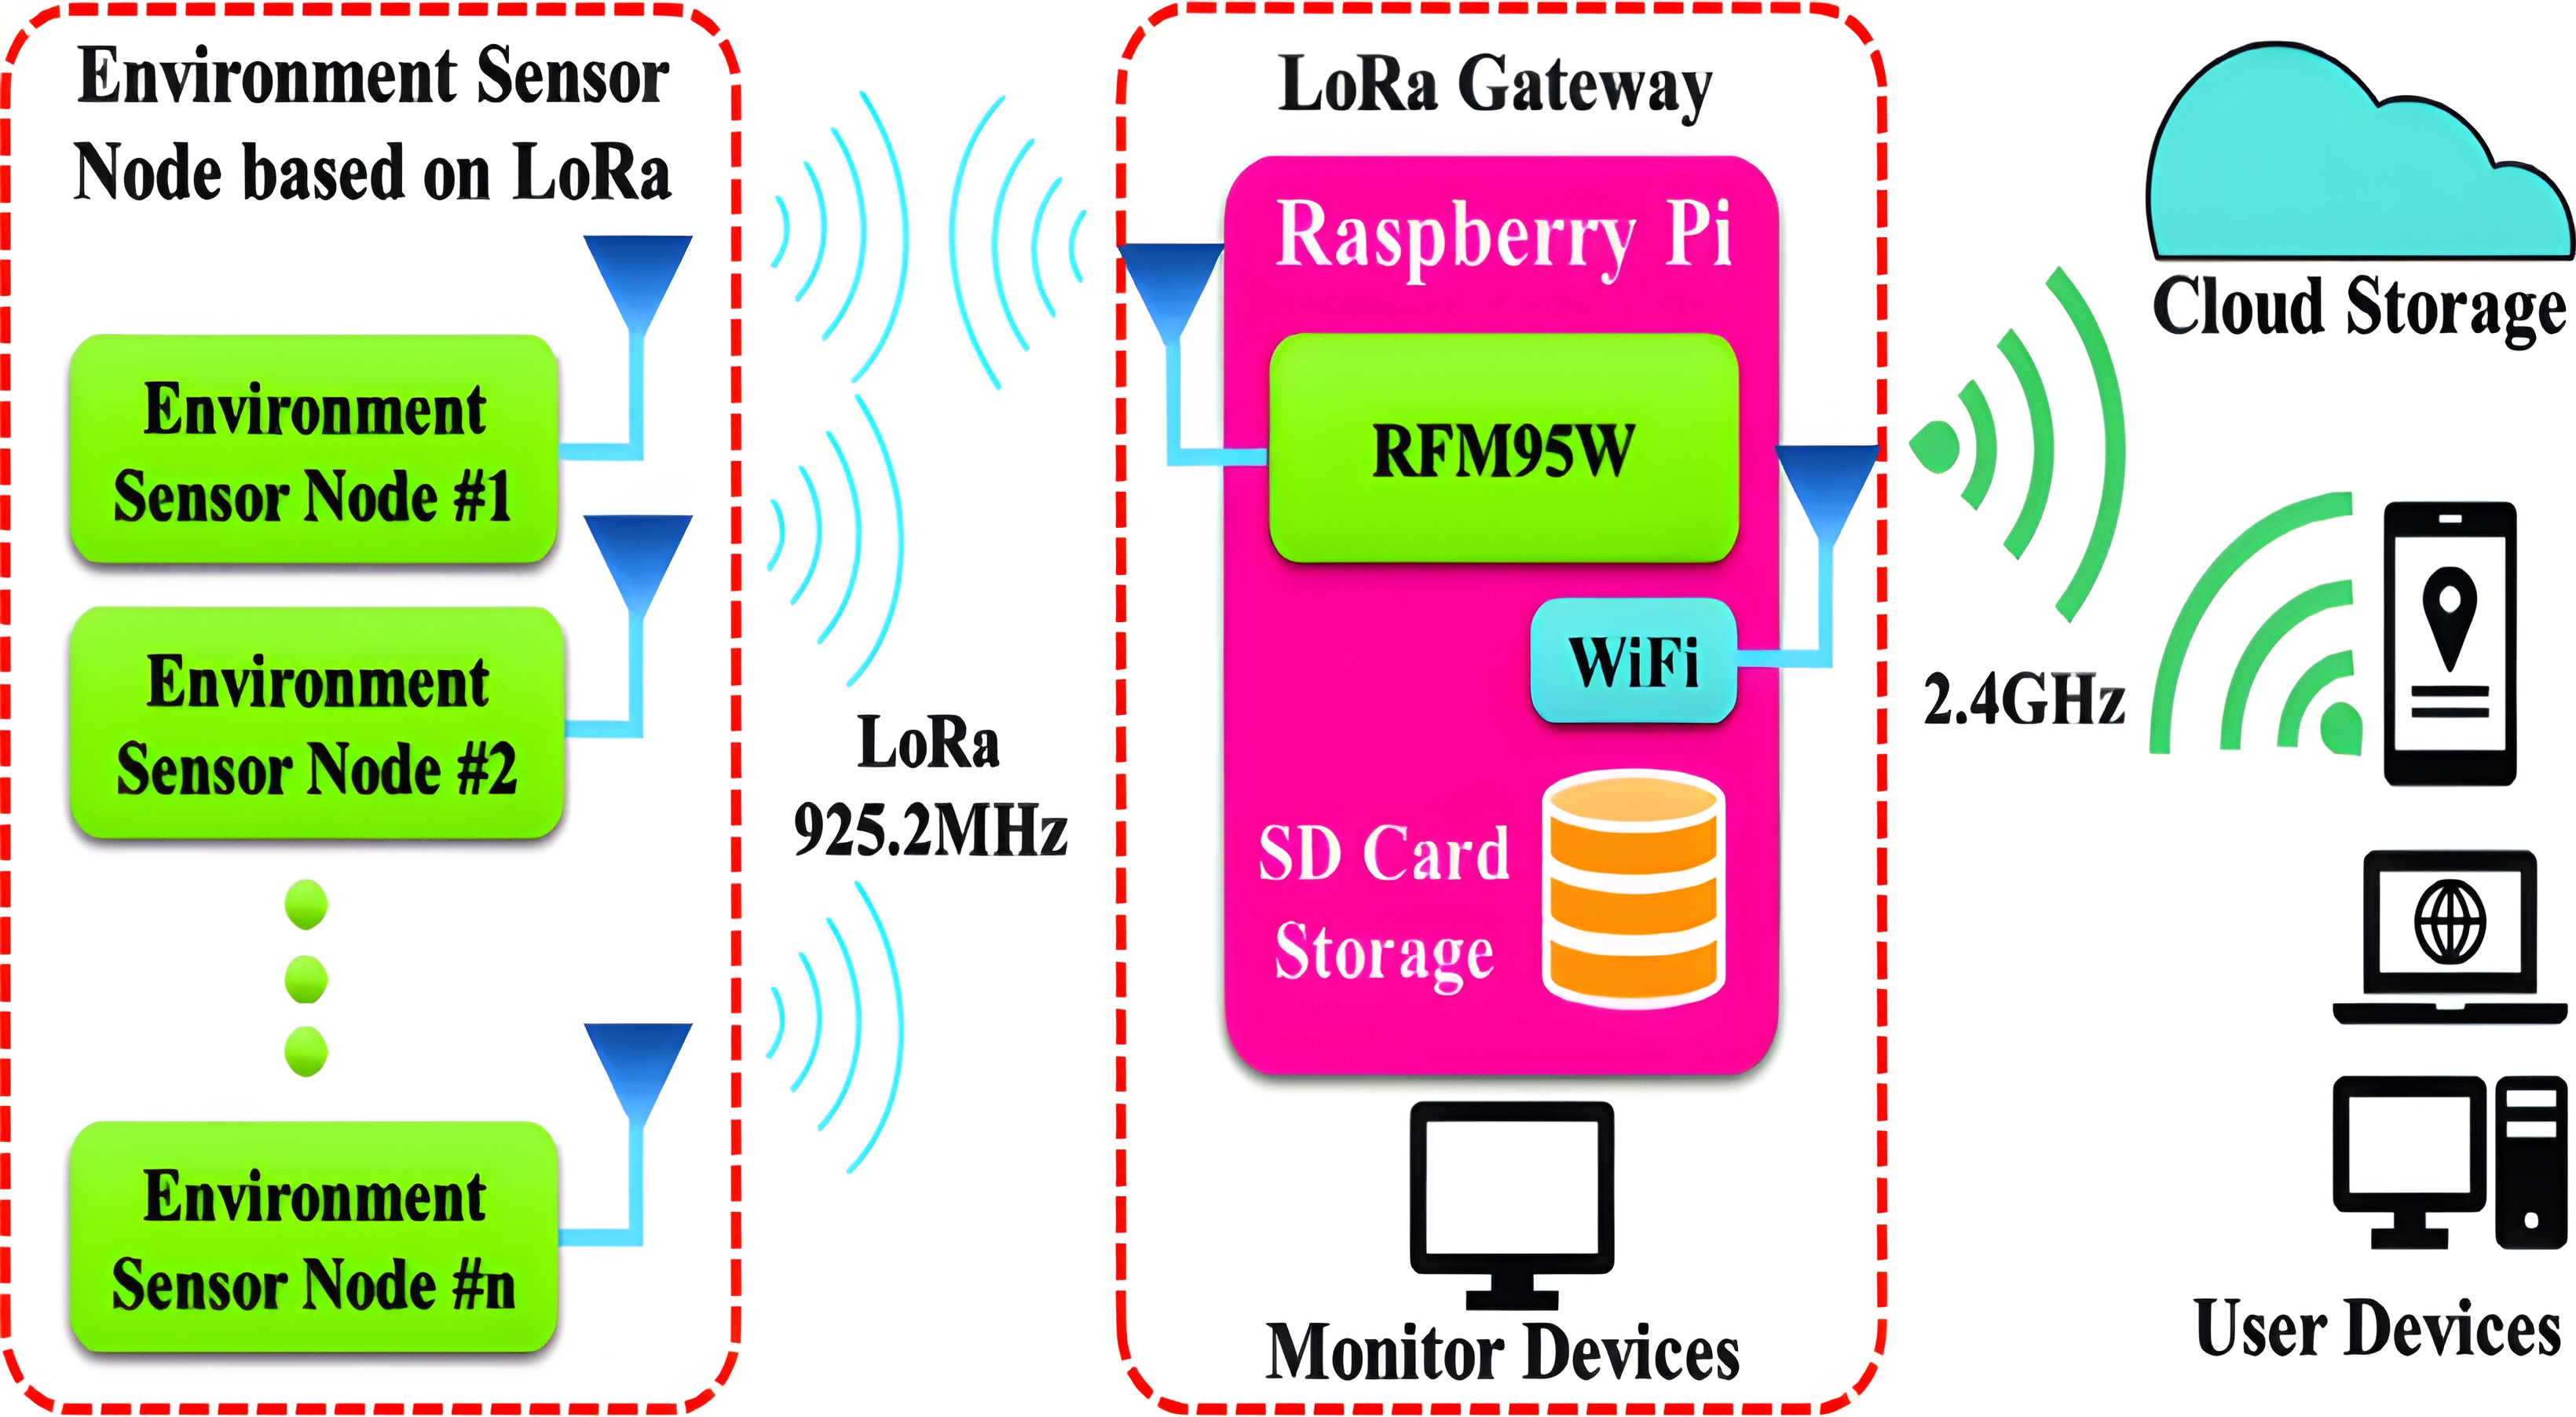
\includegraphics[scale=0.1]{Sections/Introduction/LoRaWAN-IOT-Example.jpg}
\end{figure}